% Created by tikzDevice version 0.12.3.1 on 2021-03-02 17:23:06
% !TEX encoding = UTF-8 Unicode
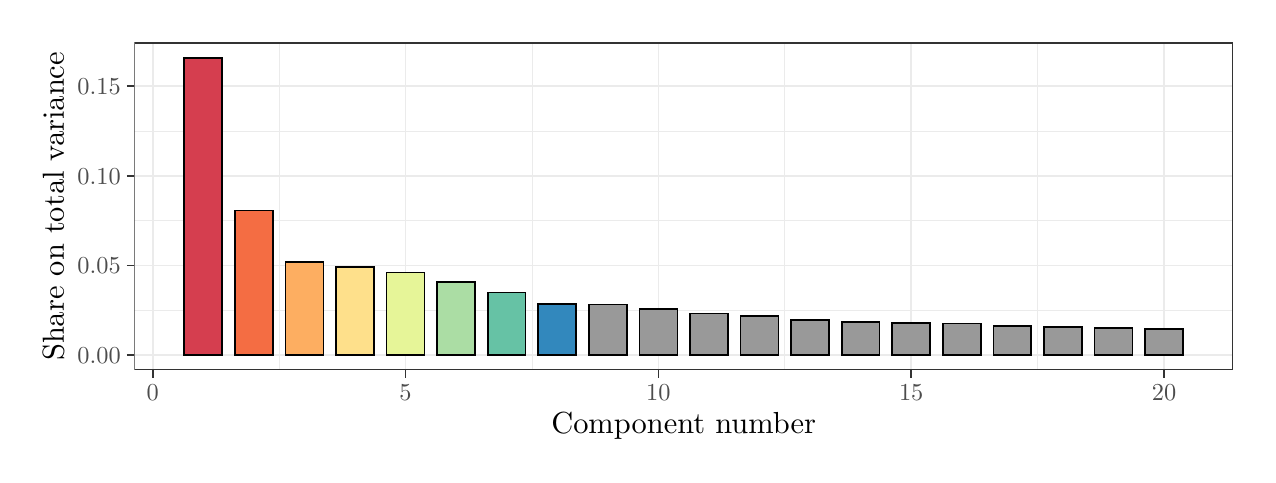
\begin{tikzpicture}[x=1pt,y=1pt]
\definecolor{fillColor}{RGB}{255,255,255}
\path[use as bounding box,fill=fillColor,fill opacity=0.00] (0,0) rectangle (441.02,154.36);
\begin{scope}
\path[clip] (  0.00,  0.00) rectangle (441.02,154.36);
\definecolor{drawColor}{RGB}{255,255,255}
\definecolor{fillColor}{RGB}{255,255,255}

\path[draw=drawColor,line width= 0.6pt,line join=round,line cap=round,fill=fillColor] (  0.00,  0.00) rectangle (441.02,154.36);
\end{scope}
\begin{scope}
\path[clip] ( 38.56, 30.69) rectangle (435.52,148.86);
\definecolor{fillColor}{RGB}{255,255,255}

\path[fill=fillColor] ( 38.56, 30.69) rectangle (435.52,148.86);
\definecolor{drawColor}{gray}{0.92}

\path[draw=drawColor,line width= 0.3pt,line join=round] ( 38.56, 52.24) --
	(435.52, 52.24);

\path[draw=drawColor,line width= 0.3pt,line join=round] ( 38.56, 84.61) --
	(435.52, 84.61);

\path[draw=drawColor,line width= 0.3pt,line join=round] ( 38.56,116.98) --
	(435.52,116.98);

\path[draw=drawColor,line width= 0.3pt,line join=round] ( 90.86, 30.69) --
	( 90.86,148.86);

\path[draw=drawColor,line width= 0.3pt,line join=round] (182.22, 30.69) --
	(182.22,148.86);

\path[draw=drawColor,line width= 0.3pt,line join=round] (273.58, 30.69) --
	(273.58,148.86);

\path[draw=drawColor,line width= 0.3pt,line join=round] (364.94, 30.69) --
	(364.94,148.86);

\path[draw=drawColor,line width= 0.6pt,line join=round] ( 38.56, 36.06) --
	(435.52, 36.06);

\path[draw=drawColor,line width= 0.6pt,line join=round] ( 38.56, 68.43) --
	(435.52, 68.43);

\path[draw=drawColor,line width= 0.6pt,line join=round] ( 38.56,100.80) --
	(435.52,100.80);

\path[draw=drawColor,line width= 0.6pt,line join=round] ( 38.56,133.17) --
	(435.52,133.17);

\path[draw=drawColor,line width= 0.6pt,line join=round] ( 45.18, 30.69) --
	( 45.18,148.86);

\path[draw=drawColor,line width= 0.6pt,line join=round] (136.54, 30.69) --
	(136.54,148.86);

\path[draw=drawColor,line width= 0.6pt,line join=round] (227.90, 30.69) --
	(227.90,148.86);

\path[draw=drawColor,line width= 0.6pt,line join=round] (319.26, 30.69) --
	(319.26,148.86);

\path[draw=drawColor,line width= 0.6pt,line join=round] (410.62, 30.69) --
	(410.62,148.86);
\definecolor{drawColor}{RGB}{0,0,0}
\definecolor{fillColor}{RGB}{213,62,79}

\path[draw=drawColor,line width= 0.6pt,line cap=rect,fill=fillColor] ( 56.60, 36.06) rectangle ( 70.30,143.48);
\definecolor{fillColor}{RGB}{244,109,67}

\path[draw=drawColor,line width= 0.6pt,line cap=rect,fill=fillColor] ( 74.87, 36.06) rectangle ( 88.58, 88.35);
\definecolor{fillColor}{RGB}{253,174,97}

\path[draw=drawColor,line width= 0.6pt,line cap=rect,fill=fillColor] ( 93.14, 36.06) rectangle (106.85, 69.74);
\definecolor{fillColor}{RGB}{254,224,139}

\path[draw=drawColor,line width= 0.6pt,line cap=rect,fill=fillColor] (111.42, 36.06) rectangle (125.12, 67.89);
\definecolor{fillColor}{RGB}{230,245,152}

\path[draw=drawColor,line width= 0.6pt,line cap=rect,fill=fillColor] (129.69, 36.06) rectangle (143.39, 65.91);
\definecolor{fillColor}{RGB}{171,221,164}

\path[draw=drawColor,line width= 0.6pt,line cap=rect,fill=fillColor] (147.96, 36.06) rectangle (161.66, 62.35);
\definecolor{fillColor}{RGB}{102,194,165}

\path[draw=drawColor,line width= 0.6pt,line cap=rect,fill=fillColor] (166.23, 36.06) rectangle (179.94, 58.68);
\definecolor{fillColor}{RGB}{50,136,189}

\path[draw=drawColor,line width= 0.6pt,line cap=rect,fill=fillColor] (184.50, 36.06) rectangle (198.21, 54.46);
\definecolor{fillColor}{gray}{0.60}

\path[draw=drawColor,line width= 0.6pt,line cap=rect,fill=fillColor] (202.78, 36.06) rectangle (216.48, 54.37);

\path[draw=drawColor,line width= 0.6pt,line cap=rect,fill=fillColor] (221.05, 36.06) rectangle (234.75, 52.69);

\path[draw=drawColor,line width= 0.6pt,line cap=rect,fill=fillColor] (239.32, 36.06) rectangle (253.02, 51.05);

\path[draw=drawColor,line width= 0.6pt,line cap=rect,fill=fillColor] (257.59, 36.06) rectangle (271.30, 50.25);

\path[draw=drawColor,line width= 0.6pt,line cap=rect,fill=fillColor] (275.86, 36.06) rectangle (289.57, 48.82);

\path[draw=drawColor,line width= 0.6pt,line cap=rect,fill=fillColor] (294.14, 36.06) rectangle (307.84, 47.90);

\path[draw=drawColor,line width= 0.6pt,line cap=rect,fill=fillColor] (312.41, 36.06) rectangle (326.11, 47.62);

\path[draw=drawColor,line width= 0.6pt,line cap=rect,fill=fillColor] (330.68, 36.06) rectangle (344.39, 47.44);

\path[draw=drawColor,line width= 0.6pt,line cap=rect,fill=fillColor] (348.95, 36.06) rectangle (362.66, 46.46);

\path[draw=drawColor,line width= 0.6pt,line cap=rect,fill=fillColor] (367.23, 36.06) rectangle (380.93, 46.27);

\path[draw=drawColor,line width= 0.6pt,line cap=rect,fill=fillColor] (385.50, 36.06) rectangle (399.20, 45.77);

\path[draw=drawColor,line width= 0.6pt,line cap=rect,fill=fillColor] (403.77, 36.06) rectangle (417.47, 45.58);
\definecolor{drawColor}{gray}{0.20}

\path[draw=drawColor,line width= 0.6pt,line join=round,line cap=round] ( 38.56, 30.69) rectangle (435.52,148.86);
\end{scope}
\begin{scope}
\path[clip] (  0.00,  0.00) rectangle (441.02,154.36);
\definecolor{drawColor}{gray}{0.30}

\node[text=drawColor,anchor=base east,inner sep=0pt, outer sep=0pt, scale=  0.88] at ( 33.61, 33.03) {0.00};

\node[text=drawColor,anchor=base east,inner sep=0pt, outer sep=0pt, scale=  0.88] at ( 33.61, 65.40) {0.05};

\node[text=drawColor,anchor=base east,inner sep=0pt, outer sep=0pt, scale=  0.88] at ( 33.61, 97.77) {0.10};

\node[text=drawColor,anchor=base east,inner sep=0pt, outer sep=0pt, scale=  0.88] at ( 33.61,130.14) {0.15};
\end{scope}
\begin{scope}
\path[clip] (  0.00,  0.00) rectangle (441.02,154.36);
\definecolor{drawColor}{gray}{0.20}

\path[draw=drawColor,line width= 0.6pt,line join=round] ( 35.81, 36.06) --
	( 38.56, 36.06);

\path[draw=drawColor,line width= 0.6pt,line join=round] ( 35.81, 68.43) --
	( 38.56, 68.43);

\path[draw=drawColor,line width= 0.6pt,line join=round] ( 35.81,100.80) --
	( 38.56,100.80);

\path[draw=drawColor,line width= 0.6pt,line join=round] ( 35.81,133.17) --
	( 38.56,133.17);
\end{scope}
\begin{scope}
\path[clip] (  0.00,  0.00) rectangle (441.02,154.36);
\definecolor{drawColor}{gray}{0.20}

\path[draw=drawColor,line width= 0.6pt,line join=round] ( 45.18, 27.94) --
	( 45.18, 30.69);

\path[draw=drawColor,line width= 0.6pt,line join=round] (136.54, 27.94) --
	(136.54, 30.69);

\path[draw=drawColor,line width= 0.6pt,line join=round] (227.90, 27.94) --
	(227.90, 30.69);

\path[draw=drawColor,line width= 0.6pt,line join=round] (319.26, 27.94) --
	(319.26, 30.69);

\path[draw=drawColor,line width= 0.6pt,line join=round] (410.62, 27.94) --
	(410.62, 30.69);
\end{scope}
\begin{scope}
\path[clip] (  0.00,  0.00) rectangle (441.02,154.36);
\definecolor{drawColor}{gray}{0.30}

\node[text=drawColor,anchor=base,inner sep=0pt, outer sep=0pt, scale=  0.88] at ( 45.18, 19.68) {0};

\node[text=drawColor,anchor=base,inner sep=0pt, outer sep=0pt, scale=  0.88] at (136.54, 19.68) {5};

\node[text=drawColor,anchor=base,inner sep=0pt, outer sep=0pt, scale=  0.88] at (227.90, 19.68) {10};

\node[text=drawColor,anchor=base,inner sep=0pt, outer sep=0pt, scale=  0.88] at (319.26, 19.68) {15};

\node[text=drawColor,anchor=base,inner sep=0pt, outer sep=0pt, scale=  0.88] at (410.62, 19.68) {20};
\end{scope}
\begin{scope}
\path[clip] (  0.00,  0.00) rectangle (441.02,154.36);
\definecolor{drawColor}{RGB}{0,0,0}

\node[text=drawColor,anchor=base,inner sep=0pt, outer sep=0pt, scale=  1.10] at (237.04,  7.64) {Component number};
\end{scope}
\begin{scope}
\path[clip] (  0.00,  0.00) rectangle (441.02,154.36);
\definecolor{drawColor}{RGB}{0,0,0}

\node[text=drawColor,rotate= 90.00,anchor=base,inner sep=0pt, outer sep=0pt, scale=  1.10] at ( 13.08, 89.77) {Share on total variance};
\end{scope}
\end{tikzpicture}
